\section{Application: Least squares approximations and curve fitting}

In this section, we will consider the problem of finding approximate
solutions to a system of linear equations $A\vect{v}=\vect{b}$. This
can be useful when the system is inconsistent, but we would still like
to find a ``best'' answer. For example, consider the following system
of equations.
\begin{equation*}
  \begin{array}{rcrcl}
    0.1 x &+& 0.2 y &=& 0.3, \\
    0.2 x &+& 0.5 y &=& 0.7, \\
    0.7 x &+& 0.2 y &=& 0.9. \\
  \end{array}
\end{equation*}
This system has the solution $(x,y)=(1,1)$, so it is clearly
consistent. Now imagine that we introduce some small inaccuracies into
the equations. The inaccuracies might perhaps be due to round-off
errors, or due to measurement errors if the coefficients are obtained
from experimental data. We might end up with the following system of
equations:
\begin{equation*}
  \begin{array}{rcrcl}
    0.1000001 x &+& 0.2 y &=& 0.3, \\
    0.2 x &+& 0.5 y &=& 0.7, \\
    0.7 x &+& 0.2 y &=& 0.9. \\
  \end{array}
\end{equation*}
Except for a tiny error in one of the coefficients, this is the same
system of equations as before. We would expect that such a small error
does not affect the result much. However, this last system of
equations is inconsistent; it has no solutions at all. You can see
this by observing that $(x,y)=(1,1)$ is still the unique solution to
the last two equations; substituting this into the first equation, we
get $0.3000001 = 0.3$, which almost, but not exactly, true. What we
would like to find in a situation like this is an ``approximate
solution'', i.e., numbers $x$ and $y$ such that each of the three
equations ``almost'' holds. We can formulate the problem more
precisely as follows:

\begin{problem}{Least squares approximation problem}{least squares-approximation}
  Given a (possibly inconsistent) system of equations
  $A\vect{v}=\vect{b}$, find $\vect{v}$ such that
  \begin{equation*}
    \norm{A\vect{v} - \vect{b}}
  \end{equation*}
  is as small as possible. We call such a vector $\vect{v}$ a
  \textbf{least squares approximation}%
  \index{least squares approximation}%
  \index{approximation!least squares} for the system of equations.
\end{problem}

To see why this is called a ``least squares'' approximation, consider
a system of equations
\begin{equation*}
  \begin{array}{c@{~}c@{~}c@{~}c@{~}c@{~}c@{~}c}
    a_{11}x_1 &+& \cdots &+& a_{1n}x_n &=& b_1, \\
    a_{21}x_1 &+& \cdots &+& a_{2n}x_n &=& b_2, \\
    \multicolumn{7}{c}{\cdots} \\
    a_{m1}x_1 &+& \cdots &+& a_{mn}x_n &=& b_m. \\
  \end{array}
\end{equation*}
We can write this in matrix form $A\vect{v}=\vect{b}$, where
\begin{equation*}
  A = \begin{mymatrix}{ccc}
    a_{11} & \cdots & a_{1n} \\
    \vdots & \ddots & \vdots \\
    a_{m1} & \cdots & a_{mn} \\
  \end{mymatrix},
  \quad
  \vect{b} = \begin{mymatrix}{c} b_1 \\ \vdots \\ b_m \end{mymatrix},
  \quad\mbox{and}\quad
  \vect{v} = \begin{mymatrix}{c} x_1 \\ \vdots \\ x_n \end{mymatrix}.
\end{equation*}
Then
\begin{equation*}
  A\vect{v} - \vect{b} ~=~
  \begin{mymatrix}{c@{~}c@{~}c@{~}c@{~}c@{~}c@{~}c}
    a_{11}x_1 &+& \cdots &+& a_{1n}x_n &-& b_1 \\
    \multicolumn{7}{c}{\cdots} \\
    a_{m1}x_1 &+& \cdots &+& a_{mn}x_n &-& b_m \\
  \end{mymatrix},
\end{equation*}
and therefore
\begin{equation*}
  \norm{A\vect{v} - \vect{b}}^2 ~=~
  (a_{11}x_1 + \cdots + a_{1n}x_n - b_1)^2 + \ldots
  + (a_{m1}x_1 + \cdots + a_{mn}x_n - b_m)^2.
\end{equation*}
Therefore, minimizing $\norm{A\vect{v}-\vect{b}}$ is the same as
minimizing the sum of the squares of the errors of all the equations,
where the error of each equation is defined to be the difference
between its left-hand side and right-hand side.

We note that $\norm{A\vect{v}-\vect{b}}=0$ if and only if
$A\vect{v}=\vect{b}$. Therefore, if the system of equations
$A\vect{v}=\vect{b}$ is consistent, then its least squares
approximations are exactly the solutions of the system of equations in
the usual sense.

The least squares approximation problem has a very elegant solution,
provided by the following proposition.

\begin{proposition}{Solution of the least squares approximation problem}{least-squares-approximation}
  A vector $\vect{v}$ is a least squares approximation of the system
  of equations $A\vect{v}=\vect{b}$ if and only if
  \begin{equation*}
    A^TA\vect{v} = A^T\vect{b}.
  \end{equation*}
\end{proposition}

\begin{proof}
  Let $\vect{a}_1,\ldots\vect{a}_n$ be the columns of the matrix
  $A$. Recall that $\sspan\set{\vect{a}_1,\ldots\vect{a}_n}$ is called
  the \textbf{column space}%
  \index{column space}%
  \index{matrix!column space} of $A$, which we write as $\col(A)$.  If
  \begin{equation*}
    \vect{v} = \begin{mymatrix}{c} x_1 \\ \vdots \\ x_n \end{mymatrix},
  \end{equation*}
  is any vector, then by the definition of matrix multiplication, we
  have
  \begin{equation*}
    A\vect{v} = x_1\vect{a}_1 + \ldots + x_n\vect{a}_n.
  \end{equation*}
  Therefore, a vector is of the form $A\vect{v}$ if and only if it is
  an element of $\col(A)$. In particular, the equation
  $A\vect{v}=\vect{b}$ has a solution if and only if $\vect{b}$ is an
  element of the column space of $A$. For $\vect{v}$ to be a least
  squares approximation, we want $\norm{A\vect{v}-\vect{b}}$ to be as
  small as possible. This means that we are looking for the element of
  $\col(A)$ that is closest to $\vect{b}$.
  \begin{center}
    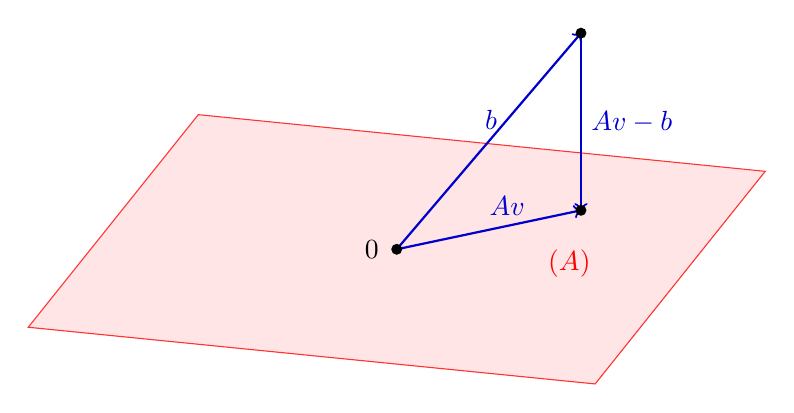
\begin{tikzpicture}[x={(1cm,-0.1cm)},y={(0.4cm,0.5cm)},z={(0cm,1cm)},scale=0.9]
      \filldraw[draw=red!80,fill=red!10](-4,-3,0) -- (4,-3,0) -- (4,3,0) -- (-4,3,0) -- cycle;
      \path[red] (2,0,0) node[right] {$\col(A)$};
      \draw[->,thick,blue!80!black](0,0,0) -- node[left, pos=0.6] {$\vect{b}$} (2,1.5,2.5);
      \draw[->,thick,blue!80!black](0,0,0) -- node[above, pos=0.6] {$A\vect{v}$} (2,1.5,0);
      \draw[->,thick,blue!80!black](2,1.5,2.5) -- node[right] {$A\vect{v}-\vect{b}$} (2,1.5,0);
      \fill (0,0,0) circle [radius=2.2pt] node [left=3pt] {$\vect{0}$};
      \fill (2,1.5,2.5) circle [radius=2.2pt];
      \fill (2,1.5,0) circle [radius=2.2pt];
    \end{tikzpicture}
  \end{center}
  From Proposition~\ref{prop:projection-subspace}, we know that this
  happens when $A\vect{v}-\vect{b}$ is orthogonal to $\col(A)$. Since
  $\col(A)=\sspan\set{\vect{a}_1,\ldots\vect{a}_n}$, this is
  equivalent to saying that $A\vect{v}-\vect{b}$ is orthogonal to each of
  the vectors $\vect{a}_1,\ldots\vect{a}_n$. Therefore,
  \begin{equation*}
    \vect{a}_i^T(A\vect{v}-\vect{b})=0
  \end{equation*}
  for $i=1,\ldots,n$. Since $\vect{a}_1^T,\ldots\vect{a}_n^T$ are the
  rows of the matrix $A^T$, this system of $n$ equations is equivalent
  to the single equation
  \begin{equation*}
    A^T(A\vect{v}-\vect{b})=\vect{0},
  \end{equation*}
  or equivalently,
  \begin{equation*}
    A^TA\vect{v} = A^T\vect{b}.
  \end{equation*}
\end{proof}

\begin{example}{Least squares approximation}{least-squares-approximation}
  Find the least squares approximation for the system of equations
  \begin{equation*}
    \begin{array}{r@{~}c@{~}r@{~}c@{~}r@{~}c@{~}r}
      2x &+& 2y &+& 2z &=&  1, \\
      x  &-&  y &-&  z &=& -2, \\
      -x &-&  y &+& 2z &=&  4, \\
      2x &+& 2y &-&  z &=& -8. \\
    \end{array}
  \end{equation*}
\end{example}

\begin{solution}
  We first write the system in matrix form $A\vect{v}=\vect{b}$, where
  \begin{equation*}
    A = \begin{mymatrix}{rrr}
      2 & 2 & 2 \\
      1 & -1 & -1 \\
      -1 & -1 & 2 \\
      2 & 2 & -1 \\
    \end{mymatrix}
    \quad\mbox{and}\quad
    \vect{b} = \begin{mymatrix}{r} 1 \\ -2 \\ 4 \\ -8 \end{mymatrix}.
  \end{equation*}
  By Proposition~\ref{prop:least-squares-approximation}, the least
  squares approximation is given by the solution of the system of
  equations $A^TA\vect{v} = A^T\vect{b}$. We calculate:
  \begin{equation*}
    A^TA =
    \begin{mymatrix}{rrrr}
      2 & 1 & -1 & 2 \\
      2 & -1 & -1 & 2 \\
      2 & -1 & 2 & -1 \\
    \end{mymatrix}
    \begin{mymatrix}{rrr}
      2 & 2 & 2 \\
      1 & -1 & -1 \\
      -1 & -1 & 2 \\
      2 & 2 & -1 \\
    \end{mymatrix}
    =
    \begin{mymatrix}{rrr}
      10 & 8 & -1 \\
      8  & 10 & 1 \\
      -1 & 1 & 10 \\
    \end{mymatrix},
  \end{equation*}
  \begin{equation*}
    A^T\vect{b} =
    \begin{mymatrix}{rrrr}
      2 & 1 & -1 & 2 \\
      2 & -1 & -1 & 2 \\
      2 & -1 & 2 & -1 \\
    \end{mymatrix}
    \begin{mymatrix}{r} 1 \\ -2 \\ 4 \\ -8 \end{mymatrix}
    =
    \begin{mymatrix}{r} -20 \\ -16 \\ 20  \end{mymatrix}.
  \end{equation*}
  Therefore, we must solve the system of equations
  \begin{equation*}
    \begin{mymatrix}{rrr}
      10 & 8 & -1 \\
      8  & 10 & 1 \\
      -1 & 1 & 10 \\
    \end{mymatrix}
    \begin{mymatrix}{c} x \\ y \\ z \end{mymatrix}
    =
    \begin{mymatrix}{r} -20 \\ -16 \\ 20  \end{mymatrix}.
  \end{equation*}
  After some row operations, we find that the unique solution is
  $(x,y,z) = (-1, -1, 2)$.  We can double-check this answer as
  follows. We calculate
  \begin{equation*}
    A\vect{v} - \vect{b}
    ~=~
    \begin{mymatrix}{rrr}
      2 & 2 & 2 \\
      1 & -1 & -1 \\
      -1 & -1 & 2 \\
      2 & 2 & -1 \\
    \end{mymatrix}
    \begin{mymatrix}{r} -1 \\ -1 \\ 2 \end{mymatrix}
    - \begin{mymatrix}{r} 1 \\ -2 \\ 4 \\ -8 \end{mymatrix}
    ~=~
    \begin{mymatrix}{r} 0 \\ -2 \\ 6 \\ -6 \end{mymatrix}
    - \begin{mymatrix}{r} 1 \\ -2 \\ 4 \\ -8 \end{mymatrix}
    ~=~ \begin{mymatrix}{r} -1 \\ 0 \\ 2 \\ 2 \end{mymatrix}
  \end{equation*}
  and check that this vector is orthogonal to every column of
  $A$. Since this is the case, our answer is correct.
\end{solution}

An important application of least squares approximations is
\textbf{curve fitting}%
\index{curve fitting}: finding the ``best'' function of a given type
(for example, linear, quadratic) to fit a given series of data points.
The next two examples show how to use least square approximations to
solve curve fitting problems.

\begin{example}{Least squares line}{least-squares-line}
  A company has collected daily data on temperature and ice cream
  sales over a period of one week. The data is as follows:
  \begin{equation*}
    \begin{array}{c@{~~~}|c|@{~~~}c}
      \mbox{Date} & \mbox{Peak temperature} & \mbox{Sales} \\\hline
      \mbox{July 1}  & 17\degC & \$320  \\    % 300 1 -5   1
      \mbox{July 2}  & 22\degC & \$570  \\    % 600 1  0  -3 -1  1  1
      \mbox{July 3}  & 26\degC & \$850  \\    % 840 1  4   1 -1 -1
      \mbox{July 4}  & 20\degC & \$470  \\    % 480 1 -2      0 -1
      \mbox{July 5}  & 24\degC & \$750  \\    % 720 1  2      2  1  1
      \mbox{July 6}  & 23\degC & \$620  \\    % 660 1  1   1       -2  1
      \mbox{July 7}  & 23\degC & \$680  \\    % 660 1  1              -1
    \end{array}
  \end{equation*}
  The company is interested in predicting how temperature will affect
  future sales. Find a function of the form $y=a+bx$ that best fits
  the data, where $x$ is temperature in degrees Celsius and $y$ is
  sales in dollars. By ``best fit'', we mean that the sum of the
  square of the errors should be as small as possible (where each
  error is the difference between the dollar amount predicted by the
  formula $y=a+bx$ and the actual dollar amount).  Such a function is
  called a \textbf{least squares line}%
  \index{least squares line}%
  \index{curve fitting!least squares line} or a \textbf{linear
    regression}%
  \index{linear regression}%
  \index{curve fitting!linear regression} for the data.
\end{example}

\begin{solution}
  We first write down a system of equations that expresses the
  relationship $y=a+bx$ for each of the seven data points $(x,y)$:
  \begin{equation*}
    \begin{array}{r@{~}c@{~}r@{~}c@{~}r}
      a &+& 17b &=& 320, \\
      a &+& 22b &=& 570, \\
      a &+& 26b &=& 850, \\
      a &+& 20b &=& 470, \\
      a &+& 24b &=& 750, \\
      a &+& 23b &=& 620, \\
      a &+& 23b &=& 680. \\
    \end{array}
  \end{equation*}
  This is a system of seven equations in two variables (the variables
  are $a$ and $b$). This system is likely inconsistent, because there
  are more equations than variables, and also because it is unlikely
  that the relationship between temperature and sales is exactly (as
  opposed to approximately) linear. Instead, we find the least squares
  approximation for the system of equations. We let
  \begin{equation*}
    A = \begin{mymatrix}{rr}
      1 & 17 \\
      1 & 22 \\
      1 & 26 \\
      1 & 20 \\
      1 & 24 \\
      1 & 23 \\
      1 & 23 \\
    \end{mymatrix}
    \quad\mbox{and}\quad
    \vect{b} =
    \begin{mymatrix}{r}
      320 \\
      570 \\
      850 \\
      470 \\
      750 \\
      620 \\
      680 \\
    \end{mymatrix}.
  \end{equation*}
  By Proposition~\ref{prop:least-squares-approximation}, we must solve
  the equation $A^TA\vect{v} = A^T\vect{b}$. We calculate
  \begin{equation*}
    A^TA = \begin{mymatrix}{cc}
      7 & 155 \\
      155 & 3483
    \end{mymatrix}
    \quad\mbox{and}\quad
    A^T\vect{b} =
    \begin{mymatrix}{c}
      4260 \\
      97380
    \end{mymatrix}.
  \end{equation*}
  So the system of equations we must solve is
  \begin{equation*}
    \begin{mymatrix}{cc}
      7 & 155 \\
      155 & 3483
    \end{mymatrix}
    \begin{mymatrix}{c} a \\ b \end{mymatrix}
    =
    \begin{mymatrix}{c}
      4260 \\
      97380
    \end{mymatrix}.
  \end{equation*}
  After some row operations, we find the unique solutions
  $(a,b)=(-720,60)$. This means that the desired linear approximation
  is $y=-720 + 60x$. The following plot shows this function along with
  the original data points.
  \begin{center}
    \begin{tikzpicture}[xscale=0.7,yscale=0.7]
      \draw[->] (15,2) -- (28,2) node[right] {$x$ (temperature)};
      \draw[->] (15,2) -- (15,10) node[above] {$y$\makebox[0in][l]{ (sales)}};
      \draw (15,2) -- +(0,-0.5) node[below] {15};
      \draw (20,2) -- +(0,-0.5) node[below] {20};
      \draw (25,2) -- +(0,-0.5) node[below] {25};
      \draw (15,2)  -- +(-0.5,0) node[left] {200};
      \draw (15,4)  -- +(-0.5,0) node[left] {400};
      \draw (15,6)  -- +(-0.5,0) node[left] {600};
      \draw (15,8)  -- +(-0.5,0) node[left] {800};
      \draw (15,10) -- +(-0.5,0) node[left] {1000};
      \fill (17,3.2) circle [radius=3.1pt];
      \fill (22,5.7) circle [radius=3.1pt];
      \fill (26,8.5) circle [radius=3.1pt];
      \fill (20,4.7) circle [radius=3.1pt];
      \fill (24,7.5) circle [radius=3.1pt];
      \fill (23,6.2) circle [radius=3.1pt];
      \fill (23,6.8) circle [radius=3.1pt];
      \draw[red,thick] (15.5,2.1) -- (27.5,9.3);
    \end{tikzpicture}
  \end{center}
  The following table compares the observed data to the computed
  linear regression (sorted by increasing temperature). It also shows
  the error for each data point.
  \begin{equation*}
    \begin{array}{c@{~~~}|c|@{~~~}c|@{~~~}c}
      \mbox{Temperature} & \mbox{Actual sales} & \mbox{Best linear fit} & \mbox{Error}\\\hline
      17 & 320 & 300 & -20 \\
      20 & 470 & 480 & +10 \\
      22 & 570 & 600 & +30 \\
      23 & 620 & 660 & +40 \\
      23 & 680 & 660 & -20 \\
      24 & 750 & 720 & -30 \\
      26 & 850 & 840 & -10 \\
    \end{array}
  \end{equation*}
  The sum of the squares of the errors is $20^2 + 10^2 + 30^2 + 40^2 + 20^2 + 30^2 + 10^2 = 4400$.
\end{solution}

\begin{example}{Least squares parabola}{least-squares-parabola}
  \index{least squares parabola}%
  \index{curve fitting!least squares parabola}
  Find a quadratic polynomial that is the best fit for the following
  data points:
  \begin{equation*}
    \begin{array}{rcr@{~}r}
      (x_1,y_1) &=& ( 3,& 23.5), \\
      (x_2,y_2) &=& ( 4,& 13.5), \\
      (x_3,y_3) &=& ( 5,& 12.5), \\
      (x_4,y_4) &=& ( 6,&  5.5), \\
      (x_5,y_5) &=& ( 7,&  9.0), \\
      (x_6,y_6) &=& ( 8,&  8.0), \\
      (x_7,y_7) &=& ( 9,& 19.0). \\
    \end{array}
  \end{equation*}
\end{example}

\begin{solution}
  We are looking for an equation of the form
  $y=a+bx+cx^2$. Substituting each of the seven data points into the
  equation, we obtain 7 equations in the unknowns $a$, $b$, and $c$:
  \begin{equation*}
    \begin{array}{r@{~}c@{~}r@{~}c@{~}rcr}
      a &+& 3b &+&  9c &=& 23.5, \\
      a &+& 4b &+& 16c &=& 13.5, \\
      a &+& 5b &+& 25c &=& 12.5, \\
      a &+& 6b &+& 36c &=&  5.5, \\
      a &+& 7b &+& 49c &=&  9.0, \\
      a &+& 8b &+& 64c &=&  8.0, \\
      a &+& 9b &+& 81c &=& 19.0. \\
    \end{array}
  \end{equation*}
  We write this in matrix form at $A\vect{v} = \vect{b}$, where
  \begin{equation*}
    A =
    \begin{mymatrix}{rrr}
      1 & 3 &  9 \\
      1 & 4 & 16 \\
      1 & 5 & 25 \\
      1 & 6 & 36 \\
      1 & 7 & 49 \\
      1 & 8 & 64 \\
      1 & 9 & 81 \\
    \end{mymatrix}
    \quad\mbox{and}\quad
    \vect{b} =
    \begin{mymatrix}{r}
      23.5 \\
      13.5 \\
      12.5 \\
      5.5 \\
      9.0 \\
      8.0 \\
      19.0 \\
    \end{mymatrix}.
  \end{equation*}
  To find the least squares approximation, we calculate
  \begin{equation*}
    A^TA = \begin{mymatrix}{ccc}
      7 & 42 & 280 \\
      42 & 280 & 2016 \\
      280 & 2016 & 15316 \\
    \end{mymatrix}
    \quad\mbox{and}\quad
    A^T\vect{b} = 
    \begin{mymatrix}{c}
      91 \\
      518 \\
      3430 \\
    \end{mymatrix}
  \end{equation*}
  and solve the system of equations $A^TA\vect{v} = A^T\vect{b}$, i.e.,
  \begin{equation*}
    \begin{mymatrix}{ccc}
      7 & 42 & 280 \\
      42 & 280 & 2016 \\
      280 & 2016 & 15316 \\
    \end{mymatrix}
    \begin{mymatrix}{c} a \\ b \\ c \end{mymatrix}
    ~=~
    \begin{mymatrix}{c}
      91 \\
      518 \\
      3430 \\
    \end{mymatrix}.
  \end{equation*}
  After doing some row operations, we find that the unique solution is
  $(a,b,c) = (67,-19,1.5)$. Therefore, the desired quadratic
  approximation is $y = 67 - 19x + 1.5x^2$. The following plot shows
  this function along with the original data points.
  \begin{center}
    \def\X{*2.0}
    \def\Y{*0.4}
    \begin{tikzpicture}[scale=0.5, domain=2.67:10, samples=50]
      \draw[->] (0\X,0\Y) -- (12\X,0\Y) node[right] {$x$};
      \draw[->] (0\X,0\Y) -- (0\X,27\Y) node[above] {$y$};
      \draw (0\X,0\Y) -- +(0,-0.5) node[below] {0};
      \draw (5\X,0\Y) -- +(0,-0.5) node[below] {5};
      \draw (10\X,0\Y) -- +(0,-0.5) node[below] {10};
      \draw (0\X,0\Y)  -- +(-0.5,0) node[left] {0};
      \draw (0\X,5\Y)  -- +(-0.5,0) node[left] {5};
      \draw (0\X,10\Y)  -- +(-0.5,0) node[left] {10};
      \draw (0\X,15\Y)  -- +(-0.5,0) node[left] {15};
      \draw (0\X,20\Y) -- +(-0.5,0) node[left] {20};
      \draw (0\X,25\Y) -- +(-0.5,0) node[left] {25};
      \fill ( 3\X, 23.5\Y) circle [radius=4.4pt];
      \fill ( 4\X, 13.5\Y) circle [radius=4.4pt];
      \fill ( 5\X, 12.5\Y) circle [radius=4.4pt];
      \fill ( 6\X,  5.5\Y) circle [radius=4.4pt];
      \fill ( 7\X,  9.0\Y) circle [radius=4.4pt];
      \fill ( 8\X,  8.0\Y) circle [radius=4.4pt];
      \fill ( 9\X, 19.0\Y) circle [radius=4.4pt];
      \draw[red,thick] plot (\x\X,{(67-19*\x+1.5*\x*\x)\Y});
    \end{tikzpicture}
  \end{center}
  The following table shows the original data, the values of the
  best fit parabola, and the error for each data point.
  \begin{equation*}
    \begin{array}{c@{~~~}|c|@{~~~}c|@{~~~}c}
      x & \mbox{Actual $y$} & \mbox{Best fit parabola} & \mbox{Error} \\\hline
      3 &  23.5 &  23.5 & ~~~0.0 \\
      4 &  13.5 &  15.0 &   +1.5 \\
      5 &  12.5 & ~~9.5 &   -3.0 \\
      6 & ~~5.5 & ~~7.0 &   +1.5 \\
      7 & ~~9.0 & ~~7.5 &   -1.5 \\
      8 & ~~8.0 &  11.0 &   +3.0 \\
      9 &  19.0 &  17.5 &   -1.5 \\
    \end{array}
  \end{equation*}
  The sum of the squares of the errors is $0^2 + 1.5^2 + 3^2 + 1.5^2 + 1.5^2 + 3^2 + 1.5^2 = 27$.
\end{solution}
